\chapter{Metode}
I dette kapitel beskrives om, hvilke metoder og processer der er anvendt igennem projektet. \\
For dybdegående beskrivelse af processen i projektet, henvises til procesrapporten som findes i bilag.

\section{ASE modellen}
Den udviklingsmodel, som primært er brugt i projektet, er ASE modellen som ses på figur \ref{fig:ASE}. ASE modellen\cite{ASE} er en mellemvægtig semi-iterativ udviklingsmodel, som er drevet ud fra en kravspecifikation, der bygger på User Stories. ASE modellen tager udgangspunkt i vandfaldsmodellen til at opbygge et projekt gennem faserne: Projektformulering - Kravspecifikation - Systemarkitektur -  Implementering -  Test/fejlfinding -  Integration og vedligeholdelse \cite{ASE}.

\begin{figure} [!ht]
	\begin{center}
		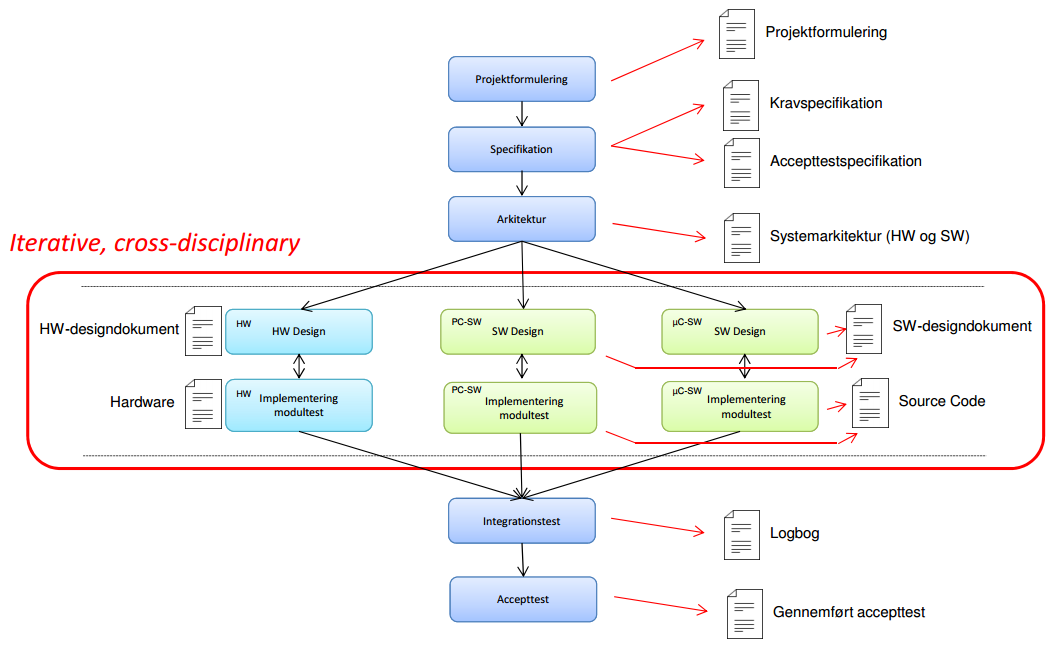
\includegraphics[height=10cm, width=12cm]{Metode/ASEModellen}
	\end{center}
	\caption{ASE modellen \cite{ASE.}}
	\label{fig:ASE}
\end{figure}

For en mere dybdegående beskrivelse af ASE modellen, se Procesrapportens Afsnit \ref{Proces-sec:ASEModel}. \\

\section{UML, Design og Test}
Der er brugt forskellige teknikker og værktøjer inden for design og test til at gennemføre projekt. Disse beskrives i afsnittene her under.
\subsection{UML}
Software designet er taget med udgangspunkt i en domænemodel og UML\cite{UML} klasse diagrammer til at vise og specificere, grænsefladerne mellem modulerne er i softwaren.
Ved hjælp af domænenmodellen udvikles softwareklasser og hvordan de interagerer med hinanden.
Domænemodellen giver et godt overblik over, hvordan de forskellige klasser skal arbejde i systemet. Derudover viser den grænseflader, som fortæller hvordan de forskellige klasser skal kommunikerre med hinanden.
Der er også udarbejdet sekvensdiagrammer, disse går under begrebet adfærdsdiagrammer som viser hvordan systemet reagerer i forskellige situationer, når brugeren interagerer med systemet.

\subsection{Design}
Software design er et værktøj, der bruges blandt udviklere til at skabe software på den bedst mulige måde. Der er mange overvejelser, der skal gøres ved valget af design. Dette bliver ofte diskuteret i grupper, for at alle er enige om, hvordan udviklingen skal gribes an og der bruges samme design fra start.

\subsection{Test}
Softwaretest bruges til at sikre en god kvalitet i koden, der bliver udviklet. Ved at skrive tests til koden, opdages fejl i kodens opførsel. Dette gør det muligt at finde fejl før udgivelse.
\newline

\section{Projektstyring}
Styringen af dette projekt, er sket gennem dagelige møder i gruppen og et ugentligt vejledermøde.
 
Der er gennem projektet blevet arbejdet iterativt med udvikling af både dokumentation, rapport og prototypen. Da gruppen har siddet samlet det meste af arbejdsprocessen er ændringer og nye tiltag blevet aftalt løbende.
Rollerne i gruppen blev før projektes start fastlagt, så man vidste hvilke ansvarsområderman havde.

Da den overordnede funktionalitet af systemet skulle bestemmes, sad gruppen og arbejdede i fællesskab, for at nå frem til et produkt der var tilfredsstillende. Gruppen har derfor været inde over kravene til systemet, og den grundlæggende opbygning af arkitekturen.
Efter alt det overordnede var blevet fastlagt, og alle var tilfredse med systemet, deltes gruppen op og arbejdede med design og implementering.
Der har været tre faste dage, hvor der blev arbejdet med projektet. Her blev ugens problemstillinger lagt op, og der blev holdt daglig stand up møde med opdateringer på, hvor langt folk var, og hvordan disse problemstillinger kunne løses. \\
Der er blevet brugt Git til at styre versionshistorikken på alle dokumenter og software. 

Da gruppen altid sad samlet, var der god kommunikation om hvor langt de forskellige opgaver var.
Dette gav en god iterativ arbejdsproces da ændringer, blev taget i fællesskab og derved vidste gruppen hele tiden hvad der skulle ske.

Der er gennem projektet brugt forskellige værktøjer. For en oversigt over disse henvises til kravspecifikationens kapitel \ref{Krav-sec:Udviklingsvaerktoejer}
